% Template for PLoS
% Version 3.4 January 2017
%
% % % % % % % % % % % % % % % % % % % % % %
%
% -- IMPORTANT NOTE
%
% This template contains comments intended
% to minimize problems and delays during our production
% process. Please follow the template instructions
% whenever possible.
%
% % % % % % % % % % % % % % % % % % % % % % %
%
% Once your paper is accepted for publication,
% PLEASE REMOVE ALL TRACKED CHANGES in this file
% and leave only the final text of your manuscript.
% PLOS recommends the use of latexdiff to track changes during review, as this will help to maintain a clean tex file.
% Visit https://www.ctan.org/pkg/latexdiff?lang=en for info or contact us at latex@plos.org.
%
%
% There are no restrictions on package use within the LaTeX files except that
% no packages listed in the template may be deleted.
%
% Please do not include colors or graphics in the text.
%
% The manuscript LaTeX source should be contained within a single file (do not use \input, \externaldocument, or similar commands).
%
% % % % % % % % % % % % % % % % % % % % % % %
%
% -- FIGURES AND TABLES
%
% Please include tables/figure captions directly after the paragraph where they are first cited in the text.
%
% DO NOT INCLUDE GRAPHICS IN YOUR MANUSCRIPT
% - Figures should be uploaded separately from your manuscript file.
% - Figures generated using LaTeX should be extracted and removed from the PDF before submission.
% - Figures containing multiple panels/subfigures must be combined into one image file before submission.
% For figure citations, please use "Fig" instead of "Figure".
% See http://journals.plos.org/plosone/s/figures for PLOS figure guidelines.
%
% Tables should be cell-based and may not contain:
% - spacing/line breaks within cells to alter layout or alignment
% - do not nest tabular environments (no tabular environments within tabular environments)
% - no graphics or colored text (cell background color/shading OK)
% See http://journals.plos.org/plosone/s/tables for table guidelines.
%
% For tables that exceed the width of the text column, use the adjustwidth environment as illustrated in the example table in text below.
%
% % % % % % % % % % % % % % % % % % % % % % % %
%
% -- EQUATIONS, MATH SYMBOLS, SUBSCRIPTS, AND SUPERSCRIPTS
%
% IMPORTANT
% Below are a few tips to help format your equations and other special characters according to our specifications. For more tips to help reduce the possibility of formatting errors during conversion, please see our LaTeX guidelines at http://journals.plos.org/plosone/s/latex
%
% For inline equations, please be sure to include all portions of an equation in the math environment.  For example, x$^2$ is incorrect; this should be formatted as $x^2$ (or $\mathrm{x}^2$ if the romanized font is desired).
%
% Do not include text that is not math in the math environment. For example, CO2 should be written as CO\textsubscript{2} instead of CO$_2$.
%
% Please add line breaks to long display equations when possible in order to fit size of the column.
%
% For inline equations, please do not include punctuation (commas, etc) within the math environment unless this is part of the equation.
%
% When adding superscript or subscripts outside of brackets/braces, please group using {}.  For example, change "[U(D,E,\gamma)]^2" to "{[U(D,E,\gamma)]}^2".
%
% Do not use \cal for caligraphic font.  Instead, use \mathcal{}
%
% % % % % % % % % % % % % % % % % % % % % % % %
%
% Please contact latex@plos.org with any questions.
%
% % % % % % % % % % % % % % % % % % % % % % % %

\documentclass[10pt,letterpaper]{article}
\usepackage[top=0.85in,left=2.75in,footskip=0.75in]{geometry}

% amsmath and amssymb packages, useful for mathematical formulas and symbols
\usepackage{amsmath,amssymb}

% Use adjustwidth environment to exceed column width (see example table in text)
\usepackage{changepage}

% Use Unicode characters when possible
\usepackage[utf8x]{inputenc}

% textcomp package and marvosym package for additional characters
\usepackage{textcomp,marvosym}

% cite package, to clean up citations in the main text. Do not remove.
\usepackage{cite}

% Use nameref to cite supporting information files (see Supporting Information section for more info)
\usepackage{nameref,hyperref}

% line numbers
\usepackage[right]{lineno}

% ligatures disabled
\usepackage{microtype}
\DisableLigatures[f]{encoding = *, family = * }

% color can be used to apply background shading to table cells only
\usepackage[table]{xcolor}

% array package and thick rules for tables
\usepackage{array}

% create "+" rule type for thick vertical lines
\newcolumntype{+}{!{\vrule width 2pt}}

% frames around boxes
\usepackage{mdframed}

% create \thickcline for thick horizontal lines of variable length
\newlength\savedwidth
\newcommand\thickcline[1]{%
  \noalign{\global\savedwidth\arrayrulewidth\global\arrayrulewidth 2pt}%
  \cline{#1}%
  \noalign{\vskip\arrayrulewidth}%
  \noalign{\global\arrayrulewidth\savedwidth}%
}

% \thickhline command for thick horizontal lines that span the table
\newcommand\thickhline{\noalign{\global\savedwidth\arrayrulewidth\global\arrayrulewidth 2pt}%
\hline
\noalign{\global\arrayrulewidth\savedwidth}}


% Remove comment for double spacing
%\usepackage{setspace}
%\doublespacing

% Text layout
\raggedright
\setlength{\parindent}{0.5cm}
\textwidth 5.25in
\textheight 8.75in

% Bold the 'Figure #' in the caption and separate it from the title/caption with a period
% Captions will be left justified
\usepackage[aboveskip=1pt,labelfont=bf,labelsep=period,justification=raggedright,singlelinecheck=off]{caption}
\renewcommand{\figurename}{Fig}

% Use the PLoS provided BiBTeX style
\bibliographystyle{plos2015}

% Remove brackets from numbering in List of References
\makeatletter
\renewcommand{\@biblabel}[1]{\quad#1.}
\makeatother

% Leave date blank
\date{}

% Header and Footer with logo
\usepackage{lastpage,fancyhdr,graphicx}
\usepackage{epstopdf}
\pagestyle{myheadings}
\pagestyle{fancy}
\fancyhf{}
\setlength{\headheight}{27.023pt}
\lhead{
\includegraphics[width=2.0in]{PLOS-submission.eps}}
\rfoot{\thepage/\pageref{LastPage}}
\renewcommand{\footrule}{\hrule height 2pt \vspace{2mm}}
\fancyheadoffset[L]{2.25in}
\fancyfootoffset[L]{2.25in}
\lfoot{\sf PLOS}

%% Include all macros below

% \newcommand{\lorem}{{\bf LOREM}}
% \newcommand{\ipsum}{{\bf IPSUM}}
\newcommand{\rulemajor}[2]{\section{#1}\label{#2}}
\newcommand{\ruleref}[1]{Rule~\ref{#1}}

%% END MACROS SECTION


\begin{document}
\vspace*{0.2in}

% Title must be 250 characters or less.
\begin{flushleft}
{\Large
\textbf\newline{Ten simple rules for collaborative lesson development} % Please use "sentence case" for title and headings (capitalize only the first word in a title (or heading), the first word in a subtitle (or subheading), and any proper nouns).
}
\newline
% Insert author names, affiliations and corresponding author email (do not include titles, positions, or degrees).
\\
{Gabriel~A.~Devenyi}\textsuperscript{1{\ddag}},
{R\'{e}mi~Emonet}\textsuperscript{2{\ddag}},
{Rayna~M.~Harris}\textsuperscript{3{\ddag}},
{Kate~L.~Hertweck}\textsuperscript{4{\ddag}},
{Damien~Irving}\textsuperscript{5{\ddag}},
{Ian~Milligan}\textsuperscript{6{\ddag}},
{Greg~Wilson}\textsuperscript{7{\ddag}*}
\\
\bigskip
\textbf{1} Douglas Mental Health University Institute, McGill University / gdevenyi@gmail.com \\
\textbf{2} Univ Lyon, UJM-Saint-Etienne, F-42023, France / remi.emonet@univ-st-etienne.fr \\
\textbf{3} The University of Texas at Austin / rayna.harris@utexas.edu \\
\textbf{4} The University of Texas at Tyler / khertweck@uttyler.edu \\
\textbf{5} CSIRO Oceans and Atmosphere / irving.damien@gmail.com \\
\textbf{6} University of Waterloo / i2millig@uwaterloo.ca \\
\textbf{7} DataCamp / gvwilson@third-bit.com \\

\bigskip

% Insert additional author notes using the symbols described below. Insert symbol callouts after author names as necessary.
%
% Remove or comment out the author notes below if they aren't used.
%
% Primary Equal Contribution Note
{\ddag} These authors contributed equally to this work.

% Additional Equal Contribution Note
% Also use this double-dagger symbol for special authorship notes, such as senior authorship.
% \ddag These authors also contributed equally to this work.

% Current address notes
% \textcurrency Current Address: Dept/Program/Center, Institution Name, City, State, Country % change symbol to "\textcurrency a" if more than one current address note
% \textcurrency b Insert second current address
% \textcurrency c Insert third current address

% Deceased author note
% \dag Deceased

% Group/Consortium Author Note
% \textpilcrow Membership list can be found in the Acknowledgments section.

% Use the asterisk to denote corresponding authorship and provide email address in note below.
* corresponding author

\end{flushleft}

% Please keep the abstract below 300 words

\linenumbers

\section*{Abstract}

Lessons take significant effort to build and maintain.
The collaborative development methods pioneered by the open source software community
offer an effective, economical way to create and sustain lessons
that can be used by large numbers of people in a wide variety of contexts.
The ten simple rules outlined in this paper
summarize the best practices that have been implemented
by several successful open education projects aimed at researchers and research librarians
in a wide range of disciplines.

% Use "Eq" instead of "Equation" for equation citations.

\section*{Introduction}

Lessons take significant effort to build and even more to maintain.
Most academics do this work on their own,
but leveraging a community approach
can make educational resource development more sustainable, robust, and responsive.
Treating lessons as a community resource
to be updated, adapted, and improved incrementally,
can free up valuable time while increasing quality.

Despite the success of openness in software development and the curation of Wikipedia,
it is an uncommon approach in the academic instructional setting.
Each year,
thousands of university lecturers teach subjects ranging from first year biology,
to graduate-level courses in Indian film.
Some use textbooks written by one or a few authors,
but beyond that,
they develop and maintain their course materials in isolation.

Given that academic research often depends on sharing, the differing
approach to developing pedagogical materials is interesting,
but the sociology and psychology behind this blind spot are beyond the scope of this paper.


The authors have many years of experience with community-developed lessons
in the context of research computing in the sciences and humanities,
through organizations like Software Carpentry and Programming Historian.
Software Carpentry was founded in 1998 to teach scientists basic computing skills,
and has since spawned two sibling organizations called Data Carpentry and Library Carpentry.
Programming Historian was founded in 2008,
and has evolved into a collaboratively-edited site providing lessons to humanities scholars.
Their guiding principles are that lessons should be:

\begin{enumerate}

\item
  open and easily accessible, and

\item
  continually maintained, refined, and improved
  by a community of contributors.

\end{enumerate}

All open education projects (e.g. massive open online courses) satisfy the first criterion by definition,
but very few satisfy the second.
In other words,
while it is common for open education projects to be occasionally updated by an individual or small team
(as happens when a new edition of a book is edited and published),
this is not the same as continuous improvement by a large community of contributors.
The ten simple rules that follow summarize what we have learned about doing that
as maintainers, editors, and reviewers of lessons used by tens of thousands of people (Fig. 1, 2).
By following these rules,
we contend that it is possible to create higher quality lessons 
than could be created by an individual or small team,
both in terms of accuracy and pedagogy.
As an added bonus, the lessons are always up-to-date 
and require less time per author to develop and maintain.

\textbf{Fig 1. Graphical abstract of ten simple rules for collaborative lesson development.} \textbf{1.} To clarify your audience, consider writing learner profiles (see Box 1). \textbf{2.} Make lessons modular by breaking them into small, single-purpose modules. \textbf{3.} Teach your instructors the best practices for developing, delivering, and maintaining lessons. \textbf{4.} Encourage and empower contributors by making the contribution process transparent and straightforward. \textbf{5} Build a community around lessons by creating opportunities for participation and mentorship. \textbf{6.} Publish new version periodically and recognize contributors by their unique identifiers (e.g., ORCID). \textbf{7.} Evaluate lessons during and after class for a complete picture of the lessons' efficacy. \textbf{8.} Reduce, re-use, or recycle lessons before creating a new one from scratch. \textbf{9.} Link to other resources that complement the lesson content. \textbf{10.} Remember that you can't please everyone in your audience or community.

\textbf{Fig 2. Collaborative open lesson development.} Following the decision to develop 
lessons, activities focus on lesson development as well as community building. 
Boxes surrounded by dotten lines represent community contributions to lessons.
Dashed arrows represent connections to activities outside the original lesson design.
The box enclosed in a dash-dotted line represents unaffiliated learning resources.

\rulemajor{Clarify your audience}{audience}

The first requirement for building lessons together is
to know whom they are being built for.
``Archaeology students'' is far too vague:
are you and your collaborators thinking of
first-year students who need an introduction to the field,
graduate students who intend to specialize in the sub-discipline that is the lesson's focus,
or someone in between?
If different contributors believe different things about prerequisite knowledge,
equipment or software required,
or how much time learners will have,
they will find it difficult to work together.

Instead of starting with learning objectives (\ruleref{practices}),
it can be helpful to write \emph{learner profiles} to clarify
the learner's general background,
what they already know,
what \emph{they} think they want to do,
how the material will help them,
and any special needs they might have.
This technique is borrowed from user interface design,
and a typical learner profile is presented in Box~1.

\rulemajor{Make lessons modular}{modular}

Every instructor's needs are different,
so build small chunks that can be re-purposed in many ways.
A university lecturer in meteorology,
for instance,
might construct a course for their students by bringing together lessons on differential equations,
fluid mechanics,
and absorption spectroscopy.
Creating courses this way shifts the instructor's burden from writing to finding and synthesizing,
which are easier if lessons clearly define what they cover (\ruleref{audience}),
and if lessons have been designed by people with a shared world-view (\ruleref{practices}).

One way to achieve this is to take existing courses and break them down into smaller, single-purpose modules
(a change which has pedagogical and administrative advantages in its own right).
When this is done,
these modules can be made more discoverable
by referencing specific points in the model curricula promulgated by many professional societies
(e.g., as learning objectives).
Smaller modules are also more approachable for new contributors (\ruleref{empower}).

\rulemajor{Teach best practices for lesson development}{practices}

Decades of pedagogical research have yielded many insights into
how best to build and deliver lessons \cite{hlw}.
Unfortunately,
many college and university faculty have little or no formal training in education \cite{brownell},
so this knowledge is rarely applied in the classroom.

Our experience is that even a brief introduction to a few key practices
helps collaborative lesson development.
If people have a shared understanding of how lessons should be developed,
it is easier for them to work together.
Less obviously,
if people have a shared model of how lessons will be \emph{used},
they are more likely to build reusable material.
Finally,
teaching people how to teach is a great way to introduce them to each other and build community (Fig. 2).

By way of example, Software Carpentry encourages its volunteers to use
the popular lesson development methodology presented by \cite{wiggins-mctighe},
whereby learning objectives and assessments are created \emph{before} any lesson materials are developed.
In particular, \emph{summative assessments} are created to determine whether the learning objectives have been met,
and \emph{formative assessments} are created to gauge learners' progress and to give them a chance to practice key skills.
The completed formative assessments are put in order and only then are the lessons written, 
with the aim of connecting each formative assessment to the next.
This method is effective in its own right,
but its greatest benefit is that it gives everyone a framework for collaboration.

An example of how to teach such pedagogical practices
is Software Carpentry's (\url{https://software-carpentry.org/}) instructor training program.
First offered in 2012,
it is now a two-day course delivered both in-person and online
\cite{lessons-learned,instructor-training,how-to-teach-programming}.
In addition to a focus on pedagogy,
the course introduces everyone who takes it to who Software Carpentry's lessons are for,
how they are delivered,
and how they are maintained.
Largely as a result of this training,
several hundred people per year now contribute to Software Carpentry's lessons.

\rulemajor{Encourage and empower contributors}{empower}

Making the process for contributing to a lesson simple and transparent
is the key to receiving contributions.
Licensing, code of conduct, governance, and the review and publication process
must all be explicit rather than implicit
to lower the social barriers to contribution.

Tools can help,
especially if they allow proposed changes to be viewed and discussed
prior to their incorporation into the lessons.
(In software development this is known as ``pre-merge review''.)
However,
some tools that are popular in open source software development have considerable up-front learning costs.
Portals like GitHub,
for example,
support everything that open lesson development needs,
but require contributors to use Git,
which has a notoriously steep learning curve \cite{git-survey}.

Complicating matters further,
some file formats make collaboration easier or more difficult.
Despite their ubiquity,
open source version control systems do not directly support review or merge
of Microsoft Office or LibreOffice file formats,
which raises an additional burden for newcomers \cite{jacobs}.
While Google Docs and wikis lack some capabilities, such as
full-fledged pre-merge review (although ``suggest mode'' 
mitigates this to some degree), 
their low barrier to entry makes them more welcoming to newcomers.

The best way to choose tools for managing lessons is
to ask potential contributors what they are comfortable with
rather than requiring \emph{them} to come to \emph{you}.
Remember also that contributing to a lesson is probably not their top priority,
and look for ways to reduce their cognitive load.
For example,
threaded discussion forums can improve the signal-to-noise ratio
by reducing long reply-all email exchanges.
Several open frameworks are available to facilitate development of new lessons,
such as learnr (\url{https://rstudio.github.io/learnr}),
Morea (\url{https://morea-framework.github.io}),
and DataCamp's templates (\url{https://www.datacamp.com/teach/documentation}).

\rulemajor{Build community around lessons}{community}

Software versions and dependencies are constantly changing,
while the academic literature is advancing at an ever-increasing pace.
As a result,
what is cutting edge one year may be out of date the next and simply wrong the year after.
Collaborative lesson development groups must therefore focus
on creating a community in which contributors support each other
rather than on relying on a small group of stewards.
Authors cannot be expected to maintain continual vigilance on a lesson,
but this is necessary for continual use.

A key part of doing this is to create opportunities for legitimate peripheral participation.
Curating a list of small tasks that newcomers can easily tackle,
encouraging them to give feedback on proposed changes,
or asking them to add new exercises and tweak diagrams and references
can all provide an on-ramp for people who might question their own authority or ability to change the main body of a lesson.
Equally,
acknowledging all contributions,
however small,
gives new contributors an early reward for taking part. 

Finally,
working in the open can be great,
but can also unintentionally suppress voices.
Programming Historian makes an ombudsperson available for private chats and facilitation
to ensure that no one is excluded. Software Carpentry operates by a Code of Conduct that outlines acceptable standards of behavior for our community members and those interacting with the Carpentries at in-person events and in virtual spaces. Community members on a 'Policy Subcommittee' serve as advocates for the CoC and adjudicate reported Code of Conduct violations. Together, the Code of Conduct and the Policy Subcommittee help ensure that all members of the community are treated with respect.

\rulemajor{Publish periodically and recognize contributions}{publish}

Like software,
specific versions of lessons should be published or released periodically
so that learners or instructors have something stable to refer to for the duration of their use (Fig. 2).
Periodic releases also provide an opportunity
for recognizing the contributions of new authors and maintainers.

Academia has only a few ways of recognizing contributions.
Until these are expanded,
it is important to publish lessons in ways that traditional academic systems can digest.
One is to give releases DOIs supplied by providers such as Zenodo (\url{https://zenodo.org/})
or DataCite (\url{https://www.datacite.org/}).
Contributors can be listed as authors
and the maintainers of the lesson as editors
to differentiate recognition of their contributions.
Each time the lesson is published,
names (and identifiers such as ORCIDs (\url{https://orcid.org}))
should be gathered for all contributors.

A lesson release is a good opportunity to bring the material into a stable shape
by fixing outstanding issues and merging contributions.
Version control automatically maintains a list of contributors,
and can also be used to track what content is in what release
(e.g., using branches or tags).
Lesson releases should use a consistent naming scheme;
Software Carpentry has used the year and month of release
(e.g., ``2017.05'')
in its releases \cite{shell2015,shell2017}.

If lessons are being released regularly,
automate the process
and archive old versions in a discoverable location.
Also make sure that everyone involved knows what ``done'' looks like,
i.e.,
which outstanding issues have to be addressed
and how they have to be formatted
in order for the next release to go out.
A simple checklist stored with the lesson materials is good enough to start,
but as time goes by,
the community may want to use an issue tracking system of some sort
so that work items can be assigned to specific people
and then ticked off as they are completed.

\rulemajor{Evaluate lessons at several scales}{evaluate}

What people immersed in developing lessons think needs fixing
can easily differ from what learners think.
It is therefore critical to gather and act on feedback at several scales
to check assumptions and stay on course (Fig. 2).

Micro-scale feedback can be gathered by an instructor while teaching a particular lesson.
Learners can provide feedback on everything from typographical errors
and the clarity of quiz questions
to the order in which topics are presented,
all of which the instructor should record at the end of each class
in some shared location (such as a Google Doc or GitHub issues).
As well as encouraging direct verbal feedback,
it's a good idea to provide learners with a means to provide feedback anonymously during class
(e.g., on small pieces of paper like sticky notes or through anonymous surveys).

Pre- and post-class surveys and interviews should be used to uncover larger issues,
particularly those arising from developers not fully understanding their audience,
e.g.,
assuming prior knowledge that learners do not have.
Post-class surveys are most effective when conducted 30--90 days after class;
this gives people time to reflect,
so their feedback will more accurately reflect what they learned
rather than how entertained they were.
Clearly-stated learning objectives (\ruleref{practices}) are essential here,
as they tell assessors what they should be measuring.

\rulemajor{Reduce, re-use, recycle}{rrr}

Just as a scholar would not write a paper without a literature review,
an instructor should not create a new lesson if there is an existing one they could use or contribute to.
A short online search can discover if someone has written what you need,
whether it is complementary to your goals,
and if it can be tweaked or modified to meet your needs.

Before re-using content,
make sure to check its license.
Both Programming Historian and the Carpentry projects
use the Creative Commons--Attribution license
(\url{https://creativecommons.org/licenses/by/4.0/}),
which allows people to share and adapt material for any purpose
as long as they cite the original source.
Other Creative Commons licenses may restrict commercial use
and/or creation of derivative materials.

The question of licensing also arises when recycling lesson components
such as images, data, figure, or code.
If the license does not cover them explicitly,
ask permission as you would for any other academic material.

The converse of this rule is to make the license for your lessons explicit and discoverable.
For example,
when lessons are published (\ruleref{publish}),
make sure that that keywords such as ``CC-BY'' appear in their bibliography entries
and HTML page headers.

\rulemajor{Link to other resources}{link}

Learners are unlikely to absorb everything they need to know about a topic from your lesson alone.
This is partly a matter of scope---any interesting subject is too large
to fit in a single lesson---but also a matter of level and direction.
As Caulfield has argued \cite{choral-explanations},
the best way to use the Internet is to provide a chorus of explanations
that offer many angles and approaches for any given topic,
each of which may be the best fit for a different set of needs (Fig. 2).

Collaboratively-developed lessons should direct learners to these resources at strategic points.
Textbooks,
technical documentation,
videos,
web pages,
threads on Quora or mailing lists:
if a community or discussion forum exists for the topic,
it is worth including.

Doing this is substantial work,
and maintaining it is even more so,
which makes building community around lessons (\ruleref{community}) all the more important.
In particular,
it is vital to engage the learners as equal participants in that community:
they should both be able to propose updates, corrections, and additions to lessons,
and know that they are encouraged to do so (\ruleref{empower}).

\rulemajor{You can't please everyone}{everyone}

No single lesson can be right for every learner.
Two people with no prior knowledge of a specific subject
may still be able to move at different speeds
because of different levels of general background knowledge.
Similarly,
lessons on ecology for learners in Utah and Vietnam
will probably be more relatable if they use different examples.
A community may therefore maintain several differently-oriented or differently-paced lessons
on a single topic,
just as programming languages provide several different libraries for doing the same general thing
with different levels of performance and complexity.

Similarly,
no lesson development community can serve all purposes.
Some groups may prioritize rapid evolution,
while others may prefer a ``measure twice, cut once'' approach.
If there are complementary ways to explain something,
or points of view that can cohabit respectfully,
it may be possible to present them side by side.
There are good pedagogical reasons to do this
even if contributors \emph{do not} disagree:
weighing alternatives fosters higher-order thinking.

But sometimes choices must be made.
The open source software community has wrestled with these issues for three decades,
and has evolved some best practices to address them
\cite{producing-oss}.
As discussed in \ruleref{empower},
the first step is to have a clear governance structure and a clear, permissive license.
Minor disagreements should be discussed openly and respectfully.
If they turn out not to be so minor after all,
contributors should split off and evolve the lesson in the way they see best.
(This is one of the reasons to have a permissive license.)

These splits rarely happen in practice.
When they do,
it is important to remember that we all share the same vision of better lessons, built together.

\section*{Conclusion}

Every day,
teachers all over the world spend countless hours duplicating each other's work.
These ten rules provide an alternative:
adopting the model of collaborative software development
to make more robust and sustainable lessons in all domains
that can be continually improved by those who use them.
We hope that our experiences can help others teach more
with more impact and less effort.

\subsection*{Acknowledgments}

We are grateful to everyone who provided feedback on this paper,
including
James Baker,
Nathan Moore,
Pariksheet Nanda,
Tom Pollard,
Byron Smith,
and Andrew Walker.
We are also grateful to the hundreds of people who have contributed to
Programming Historian, Data Carpentry, Software Carpentry, and Library Carpentry
over many years.

\nolinenumbers

% Either type in your references using
% \begin{thebibliography}{}
% \bibitem{}
% Text
% \end{thebibliography}
%
% or
%
% Compile your BiBTeX database using our plos2015.bst
% style file and paste the contents of your .bbl file
% here. See http://journals.plos.org/plosone/s/latex for
% step-by-step instructions.

\newpage

\begin{thebibliography}{1}

\bibitem{hlw}
Ambrose SA, Bridges MW, DiPietro M, Lovett MC, Norman MK.
\newblock How Learning Works.
\newblock Jossey-Bass; 2010.

\bibitem{wiggins-mctighe}
Wiggins G, McTighe J.
\newblock Understanding by Design.
\newblock 2nd ed. Association for Supervision and Curriculum Development; 2005.

\bibitem{lessons-learned}
Wilson G.
\newblock Software Carpentry: Lessons Learned.
\newblock F1000Research, 3(62), 2016,
\newblock 10.12688/f1000research.3-62.v2.

\bibitem{instructor-training}
Koch C. and Wilson G. (eds.)
\newblock Software Carpentry: Instructor Training; 2016.
\newblock \url{https://zenodo.org/record/57571#.WS8huDOZPdQ}.

\bibitem{how-to-teach-programming}
Wilson G.
\newblock How to Teach Programming (And Other Things).
\newblock Lulu.com; 2017.

\bibitem{shell2015}
Devenyi G.~A. and Koch C. (eds.):
Software Carpentry: The Unix Shell; 2015.
\newblock \url{https://zenodo.org/record/27355#.WS8lajOZPdQ}.

\bibitem{shell2017}
Devenyi G.~A. and Srinath A. (eds.):
Software Carpentry: The Unix Shell; 2017.
\newblock \url{https://zenodo.org/record/278226#.WS74tTOZPdQ}.

\bibitem{choral-explanations}
Caulfield M. Choral Explanations; 2016.
\newblock \url{https://hapgood.us/2016/05/13/choral-explanations/}.

\bibitem{producing-oss}
Fogel K.
\newblock Producing Open Source Software.
\newblock O'Reilly; 2005.

\bibitem{git-survey}
GitLab
\newblock Global Developer Survey.
\newblock \url{http://get.gitlab.com/global-developer-survey/}, 2016.

\bibitem{brownell}
Brownell S.~E. and Tanner K.~D.:
Barriers to faculty pedagogical change: Lack of training, time, incentives, and...tensions with professional identity?
\newblock CBE Life Sciences Education,
\newblock 11(4), 2012,
\newblock 10.1187/cbe.12-09-0163.

\bibitem{jacobs}
Jacobs C.~T., Gorman G.~J., Rees H.~E., and Craig L.~E.:
Experiences With Efficient Methodologies for Teaching Computer Programming to Geoscientists
\newblock Journal of Geoscience Education
\newblock 64(3),
\newblock 2016,
\newblock 10.5408/15-101.1

\end{thebibliography}

\newpage

%%%%% Figure  dissociation
\begin{figure}[ht]  % h = here, t = top, b = bottom, p = float
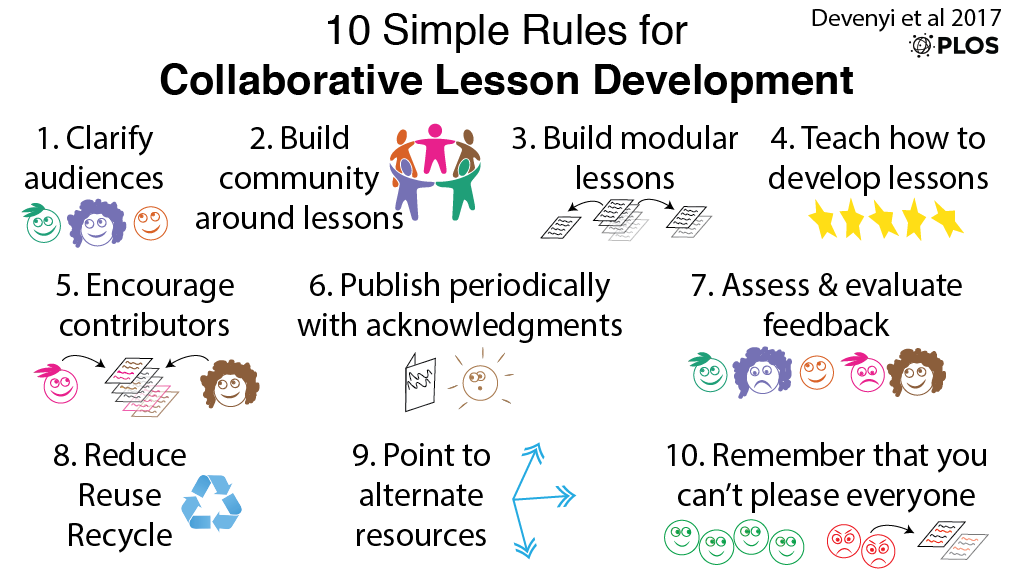
\includegraphics[width=\linewidth]{figure1}
\caption{Graphical abstract of 10 simple rules for collaborative lesson development}
\label{figure1}
\end{figure}

\newpage

%%%%% Figure  dissociation
\begin{figure}[ht]  % h = here, t = top, b = bottom, p = float

\includegraphics[width=\linewidth]{figure2}
\caption{Collaborative open lesson development}
\label{figure2}
\end{figure}

\newpage

\begin{mdframed}

\noindent
Box 1: Learner Profile

Jorge has just moved from Costa Rica to Canada to study agricultural engineering.
While fluent in both Spanish and English,
he has a hearing disability that sometimes makes it hard for him to understand lectures,
particularly in noisy environments.
Other than using Excel, Word, and the Internet,
Jorge's most significant previous experience with computers is
helping his sister build a WordPress site for the family business.

Jorge needs to measure properties of soil from nearby farms
using a handheld device that sends text files to his computer.
Right now, Jorge has to open each file in Excel,
crop the first and last points,
and calculate an average.
This workshop will show Jorge how to write a little Python program
to read the data,
select the right values from each file,
and calculate the required statistics.

\end{mdframed}

\end{document}
